%
% 24-Apq.tex
%
% (c) 2023 Prof Dr Andreas Müller
%

%
% Der Faktor A(p,q,\omega)
%
\subsection{Der Faktor $A(p,q,\omega)$}
Die im vorangegangenen Abschnitt gefundene Faktorisierung von $\mathscr{F}$
für $n=6=2\cdot 3$ lässt sich auf ein beliebiges Produkt $n=p\cdot q$ 
verallgemeinern.
Durch wiederholte Anwendung der Faktorisierung wird sich daraus später
in Abschnitt~\ref{buch:diskret:section:schnell} eine Faktorisierung
in Matrizen mit sehr wenigen Einträgen konstruieren lassen wird,
die eine schnelle Berechnung der Fouriertransformation ermöglichen
wird.

%
% Definition des Faktors
%
\subsubsection{Definition des Faktors $A(p,q,\omega)$}
Zur Konstruktion der Faktorisierung von $\mathscr{F}_n$ sei wieder
$\omega$ eine primitive $n$-te Einheitswurzel, also
$\omega^n=\omega^{pq}=1$.
Der erste Faktor der Faktorisierung ist die Matrix
\begin{equation}
\def\dx{2}
\def\dy{0.5}
\def\punkt#1#2{({(#2)*\dx},{-(#1)*\dy})}
\def\block#1#2#3{
\fill[color=red!20] \punkt{#1}{#2} rectangle \punkt{#1+1}{#2+1};
\draw[color=red] \punkt{#1}{#2} rectangle \punkt{#1+1}{#2+1};
\node at \punkt{#1+0.5}{#2+0.5} {$B_{#3}$};
}
\def\punkte#1#2{
	\fill[color=red] \punkt{#1-0.3}{#2-0.3} circle[radius=0.02];
	\fill[color=red] \punkt{#1-0.15}{#2-0.15} circle[radius=0.02];
	\fill[color=red] \punkt{#1}{#2} circle[radius=0.02];
	\fill[color=red] \punkt{#1+0.15}{#2+0.15} circle[radius=0.02];
	\fill[color=red] \punkt{#1+0.3}{#2+0.3} circle[radius=0.02];
}
A(p,q,\omega)
=
\left(\raisebox{-5.0cm}{%
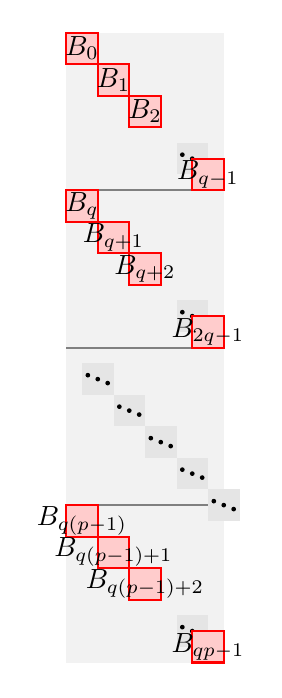
\begin{tikzpicture}[>=latex,thick]
\fill[color=gray!10] \punkt{0}{0} rectangle \punkt{20}{5};
\foreach \y in {5,10,15}{
	\draw[color=gray] \punkt{\y}{0} -- \punkt{\y}{5};
	\draw[color=gray] \punkt{\y}{0} -- \punkt{\y}{5};
	\draw[color=gray] \punkt{\y}{0} -- \punkt{\y}{5};
}
\block{0}{0}{0}
\block{1}{1}{1}
\block{2}{2}{2}
\punkte{3.5}{3.5}
\block{4}{4}{q-1}
%
\block{5}{0}{q}
\block{6}{1}{q+1}
\block{7}{2}{q+2}
\punkte{8.5}{3.5}
\block{9}{4}{2q-1}
%
\punkte{10.5}{0.5}
\punkte{11.5}{1.5}
\punkte{12.5}{2.5}
\punkte{13.5}{3.5}
\punkte{14.5}{4.5}
%
\block{15}{0}{q(p-1)}
\block{16}{1}{q(p-1)+1}
\block{17}{2}{q(p-1)+2}
\punkte{18.5}{3.5}
\block{19}{4}{qp-1}
\end{tikzpicture}}\right).
\end{equation}
Sie besteht aus $p$ übereinander angeordneten rechteckigen
$q\times pq$-Abschnitten.
In jeder Zeile eines solchen Abschnitts ist nur der Block
\begin{equation}
B_k
=
\begin{pmatrix}
1&\omega^k&\omega^{2k}&\dots&\omega^{(p-1)k}
\end{pmatrix}
\in
M_{1\times p}(\mathbb{R})
\label{buch:diskret:vandermonde:eqn:Apq}
\end{equation}
von $0$ verschieden.

%
% Zeilenvertauschungen in der Matrix A(p,q,\omega)
%
\subsubsection{Zeilenvertauschungen in der Matrix $A(p,q,\omega)$}
Durch Umordnung der Zeilen von $A(p,q,\omega)$ lässt sich die Matrix
$A(p,q,\omega)$ in die Form einer blockdiagonalen Matrix bringen.
Dies kann durch Multiplikation von links mit einer Permutationsmatrix
erreicht werden,
als mit einer Matrix, die in jeder Zeile und Spalte genau eine Eins
und sonst nur Nullen enthält.
Hat die Matrix $P$ in Zeile $i$ und Spalte $j$ eine Eins, dann ist
steht in der Zeile $i$ des Produktes $PA$ die Zeile $j$ der Matrix $A$.

Die Matrix $P(q,p)$ soll die Zeilen von $A(p,q,\omega)$ so umordnen,
dass die roten Blöcke jeweils unmittelbar untereinander zu liegen
kommen.
Dies wird erreicht durch die Matrix
\begin{equation}
P(q,p)
=
\def\dx{0.45}
\def\dy{0.45}
\def\punkt#1#2{({(#2)*\dx},{-(#1)*\dy})}
\def\eins#1#2{
	\fill[color=gray!20] \punkt{#1}{#2} rectangle \punkt{#1+1}{#2+1};
	\node at \punkt{(#1)+0.5}{(#2)+0.5} {$1\mathstrut$};
}
\def\punkte#1#2{
	\fill[color=gray!20] \punkt{#1}{#2} rectangle \punkt{#1+1}{#2+1};
	\foreach \d in {-0.7,0,0.7}{
		\fill \punkt{#1+0.5+\d*\dy*0.4}{#2+0.5+\d*\dx}
			circle[radius=0.03];
	}
}
\left(
\raisebox{-4.49cm}{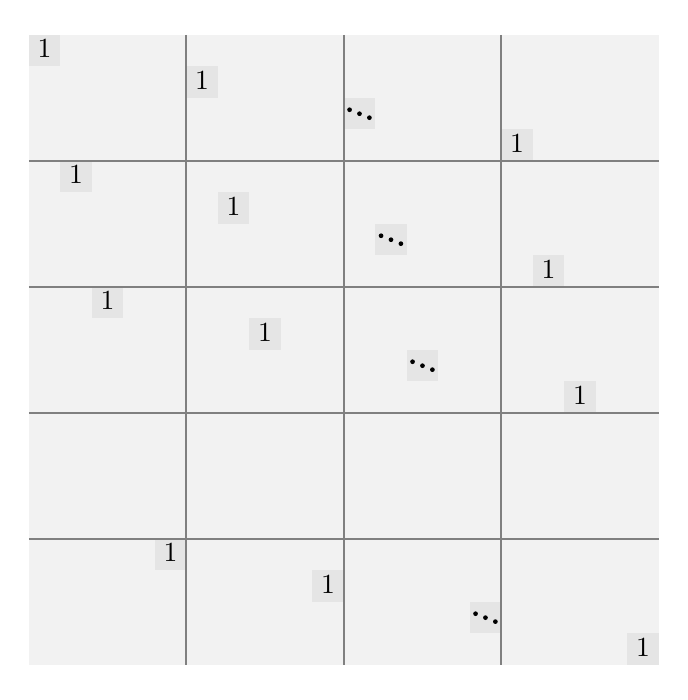
\begin{tikzpicture}[>=latex,thick]
\fill[color=gray!10] \punkt{0}{0} rectangle \punkt{20}{20};
\eins{0}{0}
\eins{1}{5}
\punkte{2}{10}
\eins{3}{15}
\eins{4}{1}
\eins{5}{6}
\punkte{6}{11}
\eins{7}{16}
\eins{8}{2}
\eins{9}{7}
\punkte{10}{12}
\eins{11}{17}
\eins{16}{4}
\eins{17}{9}
\punkte{18}{14}
\eins{19}{19}
\draw[color=gray] \punkt{4}{0} -- \punkt{4}{20};
\draw[color=gray] \punkt{0}{5} -- \punkt{20}{5};
\draw[color=gray] \punkt{8}{0} -- \punkt{8}{20};
\draw[color=gray] \punkt{0}{10} -- \punkt{20}{10};
\draw[color=gray] \punkt{12}{0} -- \punkt{12}{20};
\draw[color=gray] \punkt{16}{0} -- \punkt{16}{20};
\draw[color=gray] \punkt{0}{15} -- \punkt{20}{15};
\end{tikzpicture}}
\right).
\end{equation}
$P(q,p)$ ist eine Blockmatrix bestehend aus $q\times p$ Blöcken $B_{i\!j}$ der
Grösse $p\times q$.
Der Block $B_{i\!j}$ enthält genau eine Eines in Zeile $j$ und Spalte $i$.

\begin{definition}[Matrix $P(q,p)$]
Die Matrix $P(q,p)$ ist die Matrix mit den Einträgen
\[
(P(q,p))_{kl} = 
\begin{cases}
1\qquad&k = (i-1)p + j\;\wedge\; l= (j-1)q + i\\
0\qquad&\text{sonst}
\end{cases}
\]
für $i=1,\dots,q$ und $j=1,\dots,p$.
\end{definition}

Die Matrix $P(q,p)$ ist offenbar orthogonal, ihre Inverse ist daher
einfach die transponierte Matrix $P(q,p)^{-1}=\transpose{P(q,p)}$.
Ausserdem ist $P(q,p)^{-1}=P(p,q)$.

%
% Faktorisierung von A(p,q,\omega)
%
\subsubsection{Faktorisierung von $A(p,q,\omega)$}
Durch Multiplikation von $A(p,q,\omega)$ von links mit der Matrix $P(p,q)$
entsteht die blockdiagonale Matrix
\bgroup
\def\w{2.0}
\def\h{0.4}
\def\punkt#1#2{({(#2)*\h},{-(#1)*\h})}
\def\b#1#2#3#4#5{
	\fill[color=gray!20] \punkt{#1}{#1} rectangle \punkt{#1+5}{#1+5};
	\foreach \y in {0,1,2,4}{
		\fill[color=red!10]
			\punkt{#1+\y}{#1} rectangle \punkt{#1+\y+1}{#1+5};
		\draw[color=red] \punkt{#1+\y+1}{#1}
			-- ++\punkt{-1}{0} -- ++\punkt{0}{5} -- ++\punkt{1}{0};
	}
	\draw[color=red] \punkt{#1+3}{#1} -- \punkt{#1+3}{#1+5};
	\draw[color=red] \punkt{#1+5}{#1} -- \punkt{#1+5}{#1+5};
	\node[color=red] at \punkt{#1+3.5}{#1+2.5} {$\dots$};
	\node at \punkt{#1+0.5}{#1+2.5} {$#2$};
	\node at \punkt{#1+1.5}{#1+2.5} {$#3$};
	\node at \punkt{#1+2.5}{#1+2.5} {$#4$};
	\node at \punkt{#1+4.5}{#1+2.5} {$#5$};
}
\begin{equation}
P(q,p)\cdot A(p,q,\omega)
=
\left(\raisebox{-3.99cm}{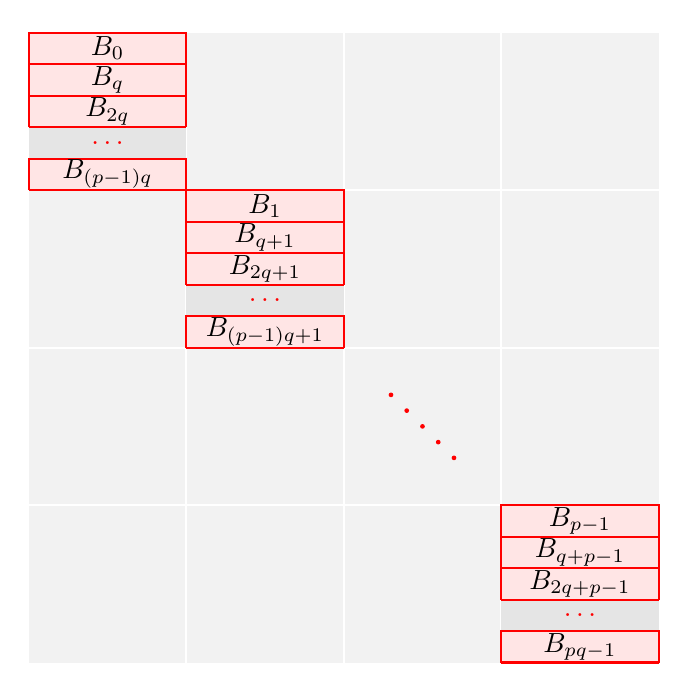
\begin{tikzpicture}[>=latex,thick]
\fill[color=gray!10] \punkt{0}{0} rectangle \punkt{20}{20};
\foreach \x in {5,10,15}{
	\draw[color=white] \punkt{\x}{0} -- \punkt{\x}{20};
	\draw[color=white] \punkt{0}{\x} -- \punkt{20}{\x};
}
\b{0}{B_0}{B_q}{B_{2q}}{B_{(p-1)q}}
\b{5}{B_1}{B_{q+1}}{B_{2q+1}}{B_{(p-1)q+1}}
\b{15}{B_{p-1}}{B_{q+p-1}}{B_{2q+p-1}}{B_{pq-1}}
\foreach \x in {-2,-1,0,1,2}{
	\fill[color=red] \punkt{12.5+\x*0.5}{12.5+\x*0.5} circle[radius=0.03];
}
\end{tikzpicture}}\right).
\label{buch:diskret:faktorisierung:eqn:PpqApq}
\end{equation}
\egroup
Der Block in der linken oberen Ecke ist eine $p$-dimensionale
Fourier-Transformation $\mathscr{F}_p$.
Die anderen Blöcke unterscheiden sich von $\mathscr{F}_p$ dadurch,
dass die Spalten mit den Elementen in der ersten Zeile multipliziert
werden.
Der Block, der mit der Zeile $B_k$ beginnt hat deher die Form
\[
\mathscr{F}_p
\cdot
\begin{pmatrix}
1&        &           &      &               \\
 &\omega^k&           &      &               \\
 &        &\omega^{2k}&      &               \\
 &        &           &\ddots&               \\
 &        &           &      &\omega^{(q-1)k}
\end{pmatrix}
=
\mathscr{F}_p\cdot \operatorname{diag}{B_k}.
\]
Setzt man diese Blöcke mit Hilfe des Kronecker-Produktes zusammen, erhält
man die Faktorisierung
\[
P(q,p)A(p,q,\omega)
=
(\mathscr{F}_p\otimes I_q)
\operatorname{diag}(B_0,B_1,\dots,B_{p-1})
\]
erhalten.

\begin{definition}[Matrix $D(p,q,\omega)$]
Die Matrix $D(p,q,\omega)$ ist die Blockdiagonalmatrix mit $p$ diagonalen
$q\times q$-Blöcken
\[
\operatorname{diag}(
B_k
)
=
\begin{pmatrix}
1&        &           &      &               \\
 &\omega^k&           &      &               \\
 &        &\omega^{2k}&      &               \\
 &        &           &\ddots&               \\
 &        &           &      &\omega^{(q-1)k}
\end{pmatrix}.
\]
\end{definition}

Unter Verwendung von $P(q,p)^{-1}=P(p,q)$ folgt der folgende Satz.

\begin{satz}[Faktorisierung von $A(p,q,\omega)$]
Die Matrix $A(p,q,\omega)$ lässt sich faktorisieren als
\begin{equation}
A(p,q,\omega)
=
P(p,q)
\cdot
(\mathscr{F}_p\otimes I_q)
\cdot
D(p,q,\omega).
\label{buch:diskret:faktorisierung:eqn:Afaktorisierung}
\end{equation}
\end{satz}

%
% Die Determinante von $A(p,q,\omega)$
%
\subsubsection{Die Determinante von $A(p,q,\omega)$}
Die Determinante von $A(p,q),\omega)$ kann explizit berechnet werden.

%
% Hauptsatz über die Matrix A(p,q,\omega)
%
\begin{satz}[Determinante von $A(p,q,\omega)$]
\label{buch:diskret:vandermonde:hauptsatz}
Die Matrix $A(p,q,\omega)$ ist regulär und hat die Determinante
\begin{equation}
\det A(p,q,\omega)
=
(-\omega)^{p(p-1)q(q-1)/4}
(\mathscr{F}_p)^q.
\label{buch:diskret:vandermonde:eqn:detA}
\end{equation}
\end{satz}

\begin{proof}[Beweis]
Mit Hilfe der Faktorisierung 
\eqref{buch:diskret:faktorisierung:eqn:Afaktorisierung}
folgt
\begin{align*}
\det A(p,q,\omega)
&=
\det P(p,q)
\det (\mathscr{F}_p\otimes I_q)
\det D(p,q,\omega)
\\
&=
\sigma(p,q) (\det\mathscr{F}_p)^q \det D(p,q,\omega).
\end{align*}
Der Faktor $\sigma(p,q)=\det P(p,q)$ wird weiter unten in
Satz~\eqref{buch:diskret:faktorisierung:satz:vorzeichen}
berechnet, der Faktor $\det D(p,q,\omega)$ in
Satz~\eqref{buch:diskret:faktorisierung:satz:detD}.
Aus den Resultaten dieser Sätze folgt die Behauptung.
\end{proof}

\begin{satz}
\label{buch:diskret:faktorisierung:satz:detD}
Die Determinanten von $D(p,q,\omega)$ ist
\[
\det D(p,q,\omega)
=
\omega^{\frac{(p-1)p(q-1)q}4}.
\]
\end{satz}

\begin{proof}[Beweis]
Wir berechnen zunächst die Determinante der Blockmatrix $B_k$:
\begin{align*}
\det \operatorname{diag}B_k
&=
1\cdot \omega^k\cdot \omega^{2k} \cdot \ldots \cdot \omega^{(q-1)k}
\\
&=
\omega^{0+k+2k+\dots+(q-1)k}
=
\omega^{k\sum_{i=0}^{q-1}i}
=
\omega^{k\frac{(q-1)q}2}.
\end{align*}
Daraus lässt sich jetzt die Determinante von $D(p,q,\omega)$ bestimmen:
\begin{align*}
\det D(p,q,\omega)
&=
\det B_0\det B_1\cdot\ldots\cdot B_{p-1}
\\
&=
\omega^{k\frac{(q-1)q}2}
\cdot
\omega^{\frac{(q-1)q}2}
\cdot
\omega^{2\frac{(q-1)q}2}
\cdot
\ldots
\cdot
\omega^{(p-1)\frac{(q-1)q}2}
\\
&=
\prod_{j=0}^{p-1}
\omega^{\frac{(q-1)q}2j}
=
\omega^{(0+1+\dots+(p-1))\frac{(q-1)q}2}
=
\omega^{\frac{(p-1)p(q-1)q}4}
\end{align*}
Damit ist der Satz bewiesen.
\end{proof}

%
% Der Vorzeichenfaktor
%
\subsubsection{Der Vorzeichenfaktor $\sigma(p,q)$}

%
% Satz über den Vorzeichenfaktor
%
\begin{satz}[Vorzeichenfaktor $\sigma(p,q)$]
\label{buch:diskret:faktorisierung:satz:vorzeichen}
Der Vorzeichenfaktor $\sigma(p,q)$
in~\eqref{buch:diskret:vandermonde:eqn:detA}
ist
\[
\sigma(p,q)
=
(-1)^{p(p-1)q(q-1)/4}.
\]
\end{satz}

\begin{proof}[Beweis]
Die Matrix $A(p,q,\omega)$ besteht aus $p$ horizontalen Blöcken mit den
Dimensionen $q\times p$.
Die $p$ Zeilen $q+1, 2q+1,\dots, (p-1)q+1$ müssen durch Vertauschungen
in die Position $2,3,\dots,p$ gebracht werden.
Wir bezeichnen die Anzahl der dafür notwendigen Vertauschungen mit
$t(p,q)$.

Um den Zeile $q+1$ in die Position $2$ zu bringen, sind $q-1$ 
Vertauschungen übereinander stehender Zeilen nötig.
Um die Zeile $2q+1$ in die Position $3$ zu bringen, sind
zunächst Vertauschungen mit den $q-1$ verbliebenen Zeilen des zweiten
Abschnittes nötig, anschliessend folgen noch $q-1$ Vertauschungen mit
den Zeilen des ersten Abschnittes.
Jeder weitere Abschnitt braucht $q-1$ zusätzliche Vertauschungen mit
den Zeilen des unmittelbar darüber liegenden Abschnittes.
Die Gesamtzahl der Vertauschungen ist daher
\[
t(p,q)
=
(q-1) + 2(q-1) + \dots +(p-1)(q-1)
=
(q-1)
\sum_{k=0}^{p-1} k
=
(q-1)\frac{p(p-1)}{2}.
\]
Damit sind die roten Blöcke in der ersten Spalte am richtigen Ort.

Nach Abschluss der Vertauschungen zur korrekten Platzierung der
roten Blöcke in der ersten Spalte bleibt eine Determinante der Form
\[
\def\w{2.0}
\def\h{0.4}
\def\punkt#1#2{({(#2)*\w},{-(#1)*\h})}
\def\b#1#2#3{
	\fill[color=red!10] \punkt{#1}{#2} rectangle \punkt{#1+1}{#2+1};
	\draw[color=red] \punkt{#1}{#2} rectangle \punkt{#1+1}{#2+1};
	\node at \punkt{#1+0.5}{#2+0.5} {$#3$};
}
\def\punkte#1#2{
	\foreach \x in {-0.2,-0.1,0,0.1,0.2}{
		\draw[color=red]
			\punkt{#1+0.5+\x}{#2+0.5+\x} circle[radius=0.01];
	}
}
\def\B#1#2{
	\fill[color=red!10,opacity=0.5]
		\punkt{#1}{#2} rectangle \punkt{#1+1}{#2+1};
}
\left|\raisebox{-3.99cm}{\begin{tikzpicture}[>=latex,thick]
\fill[color=gray!10] \punkt{0}{0} rectangle \punkt{20}{5};
\fill[color=blue!10] \punkt{4}{1} rectangle \punkt{20}{5};
\foreach \y in {4,8,12,16}{
	\draw[color=white] \punkt{\y}{0} -- \punkt{\y}{5};
}
\foreach \x in {1,2,3,4}{
	\draw[color=white] \punkt{0}{\x} -- \punkt{20}{\x};
}
\fill[color=gray!20] \punkt{2}{0} rectangle \punkt{3}{1};
\node[color=red] at \punkt{2.5}{0.5} {$\dots$};
\b{0}{0}{B_0}
\b{1}{0}{B_q}
\punkte{2}{0}
\b{3}{0}{B_{(p-1)q}}
%
\b{4}{1}{B_1}
\b{8}{1}{B_{q+1}}
\B{12}{1}
\punkte{12}{1}
\b{16}{1}{B_{(p-1)q+1}}
%
\b{5}{2}{B_2}
\b{9}{2}{B_{q+2}}
\B{13}{2}
\punkte{13}{2}
\b{17}{2}{B_{(p-1)q+2}}
%
\punkte{6}{3}
\punkte{10}{3}
\punkte{14}{3}
\punkte{18}{3}
%
\b{7}{4}{B_{p-1}}
\b{11}{4}{B_{q+p-1}}
\B{15}{4}
\punkte{15}{4}
\b{19}{4}{B_{pq-1}}
\end{tikzpicture}}\right|
\]
übrig.
Der blau hinterlegte Teil besteht wieder aus $p$ Abschnitten,
die aber nur noch $q-1$ Zeilen enthalten.
Um die roten Blöcke in der ersten Spalte des blauen Teils
nach oben zu bringen, sind daher $t(p,q-1)$ Vertauschungen nötig.

Die Gesamtzahl der Vertauschungen
\begin{align*}
t(p,q) + t(p,q-1) + \dots + t(p,2)
&=
\sum_{k=2}^q t(p,k)
=
\sum_{k=2}^q (k-1)\frac{p(p-1)}2
=
\biggl(\sum_{k=1}^{q-1} k\biggr) \frac{p(p-1)}2
\\
&=
\frac{q(q-1)}{2}\frac{p(p-1)}2.
\end{align*}
Der Vorzeichenfaktor ist daher
\[
\sigma(p,q)
=
(-1)^{q(q-1)p(p-1)/4},
\]
wie behauptet.
\qedhere
\end{proof}

